%!TEX program = xelatex
% 完整编译: xelatex -> biber/bibtex -> xelatex -> xelatex
\documentclass[lang=cn,a4paper,newtx]{elegantpaper}

\title{A2赛题: 软件功能需求分析报告}
\author{荀阳霖	\\ 韶关学院 \and 程家骏 \\ 华中科技大学 \and 刘思辰\\ 华中科技大学 \and 龚言龙 \\ 华中科技大学}
\institute{\href{https://elegantlatex.org/}{porter项目组}}

\version{1.0}
\date{\zhdate{2023/7/5}}

% 本文档命令
\usepackage{array}
\newcommand{\ccr}[1]{\makecell{{\color{#1}\rule{1cm}{1cm}}}}
\addbibresource[location=local]{reference.bib} % 参考文献,不要删除

\begin{document}

\maketitle

\begin{abstract}
    雷鸟是一个免费的邮件应用程序,可以方便地进行日程的管理,邮件的发送,thunderbird78相比与之前的版本增加了一些新的功能,如内置电子邮件加密和数字签名的功能等。
为loongarch架构移植thunderbird78或者以上版本可以帮助丰富loongarch架构的生态,提高用户的使用体验。
\keywords{loongarch, thunderbird, 软件移植}
\end{abstract}

\section{任务介绍}

A2的赛题主要任务是为loongarch架构移植thunderbird78或者以上的版本,并将其打包为deb包。
\subsection{所移植thunderbird信息}

本次移植的雷鸟版本为114.0b6,由mozilla公司进行开发,具体信息如图\ref{thunderbird}所示
\begin{figure}[!htb]
    \centering
    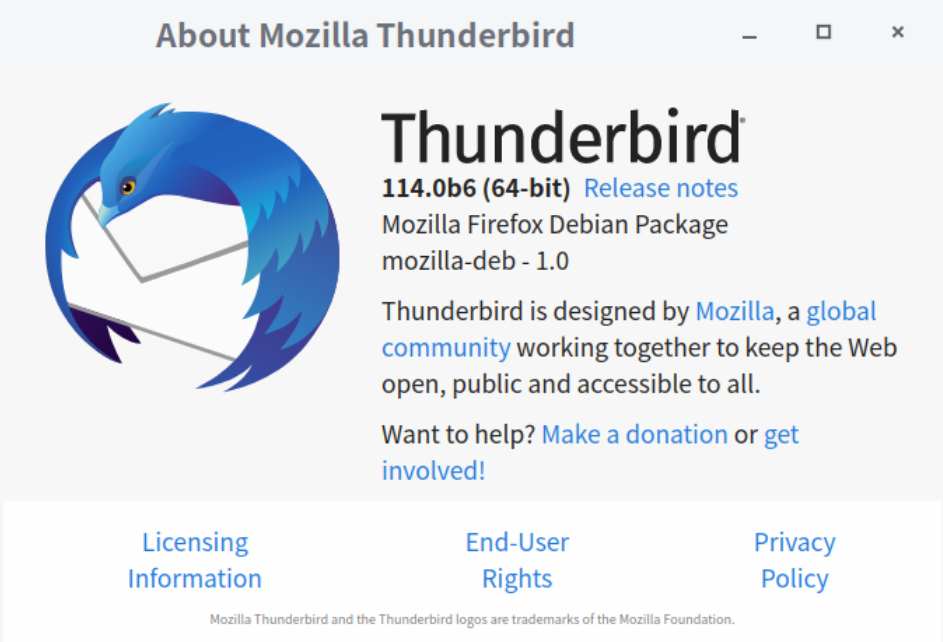
\includegraphics[width=0.6\textwidth]{thunderbird.png}
    \caption{thunderbird信息}
    \label{thunderbird}
\end{figure}

\subsection{功能需求}
\begin{enumerate}
    \item 能够在loongarch架构的机器上正常运行
    \item 通过testing目录下的测试样例
    \item 版本信息应该在78或者以上
\end{enumerate}
\subsection{开发环境}

loongnix操作系统,cpu型号3C5000L, cpu核数4核,4G内存,100G硬盘,进行fetch后得到的系统信息如图\ref{neofetch} 所示。

\begin{figure}[!htb]
    \centering
    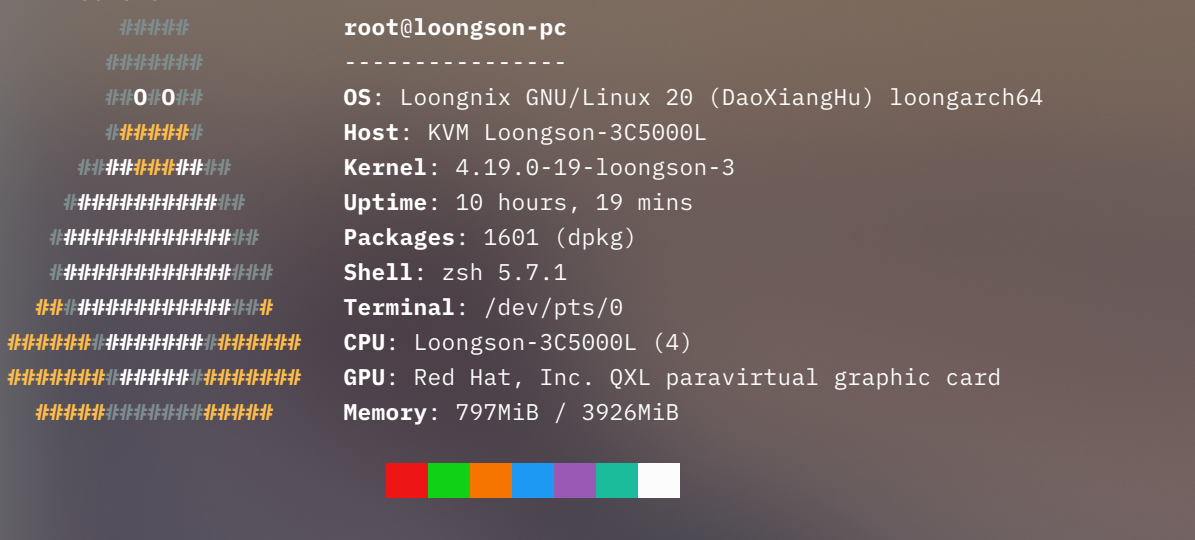
\includegraphics[width=0.8\textwidth]{fetch.png}
    \caption{neofetch结果}
    \label{neofetch}
\end{figure}


\section{软件移植记录}
\subsection{依赖适配}

编译thunderbird114及运行测试依赖于rustc1.68以上, 以及gcc13以上的版本

\subsubsection{rustc1.71.0-dev移植}
Loongarch已于24日进入Tier2。从5-25日开始,原版的rustup将提供nightly版的原生Loongarch rust工具链。从rust1.71开始,rustup将提供stable版本的原生Loongarch rust工具链

但是由于loongarch新旧世界的问题,无法直接使用最新的rust,需要在主机上进行交叉编译。

从rust仓库克隆1.71.0-dev到本地后,修改config.toml(rust配置文件),使得产出loongarch架构的二进制包。

尽管loongnix的仓库中提供了loongnix1.65的rust,但是经过对比发现主线中的rust增加了对于loongarch的特定优化。

\subsubsection{gcc-13 移植}

gcc-13的移植较为顺利,从debian sid的源中直接获取到gcc-13deb包的源码包后,修改源码包中的debian/rules文件即可,在其中仅保留对c, c++语言的支持,同时关闭对32位的支持,如果开启对其他语言的支持,
将需要编译deb中的libffi,但是其中的libffi的版本为3.4.1,未引入对于loongarch架构的支持,3.4.3中引入了对于loongarch架构的支持,但是其需要的autoconf2.71,与gcc-13所需求的的2.69相互冲突。

在编译雷鸟的过程中,仅开启对于c, c++的支持即可完成编译。

\subsubsection{llvm16.4移植}

当我们移植了gcc-13到本地之后,llvm的编译工作十分简单,只需要将llvm克隆到本地后进行编译即可。

\subsection{雷鸟打包}

修改雷鸟配置文件如下所示
\begin{lstlisting} 
    ac_add_options --enable-application=comm/mail
    ac_add_options --disable-crashreporter
    ac_add_options --without-wasm-sandboxed-libraries
    ac_add_options --enable-official-branding
    export MOZILLA_OFFICIAL=1
\end{lstlisting}

随后使用thunderbird和loongarch相关的patch,随后使用mach build进行编译

修改python/mozbuild/mozbuild/repackaging/deb.py 在\_DEB\_ARCH中增加loongarch64的相关信息

\begin{lstlisting}
    _DEB_ARCH = {
            "all": "all",
            "x86": "i386",
            "x86_64": "amd64",
            "loongarch": "loongarch64"
        }
\end{lstlisting}

同时修改browser/installer/linux/debian内和rules相关的信息
\begin{enumerate}
    \item install.in 把 firefox 修改成 thunderbird
    \item links.in 把 firefox 修改成 thunderbird
\end{enumerate}

\section{软件使用}

如果需要使用我们的移植的thunderbird-114,那么此时需要将我们上传的
thunderbird-114.0b6.source.tar.xz以及thunderbird-default\_114.0~build1\_all.deb放入到deb软件源中
的对应位置。

如果您使用的dak等软件源搭建工具,进行合理的配置后将可以使得其进行自动的数据更新。
\section{致谢}

感谢LA UOSC社区对我们相关问题的回应,以及debian中文社区对deb打包相关问题的回复

\nocite{*}
\printbibliography[heading=bibintoc, title=\ebibname]

\appendix
%\appendixpage
\addappheadtotoc

\end{document}
